
\chapter{Ambiente e resultados experimentais}
\label{cap:testes}


O sistema desenvolvido foi avaliado através da realização de experiências práticas.
Para viabilizar tal demonstração, foi desenvolvido um protótipo virtual utilizando o software Mininet \cite{website:mininet}. Mininet possibilita criar uma rede virtual escalável utilizando comutadores Open vSwitch \cite{Pfaff:2009} através de um simples \textit{script} em Python\cite{Python:2017}, facilitando a configuração de comutadores, bem como também, das conexões entres os mesmos. Além disso, Mininet possibilita a adição de \textit{hosts} virtuais com as mesmas funcionalidades do \textit{host} hospedeiro, tornando possível a criação de servidores \gls{web}, de banco de dados, testes de comunicação entre computadores e testes de ataque à servidores.
O plano de controle por sua vez é executado pelo controlador OpenDaylight \cite{website:odl} sob uma máquina física, sendo a comunicação entre o mesmo e os comutadores estabelecida através do próprio \textit{software} Mininet.


\section{Topologia de rede}

A topologia de rede adotada nos testes é modelada de maneira bem simplificada. 
Um controlador \gls{sdn} OpenDaylight realiza o gerenciamento de quatro \textit{switches} OpenFlow virtuais que por sua vez, realizam a interconexão entre servidores com serviços ativos para recepção de ataques, e computadores de uso geral que são utilizados para a realização das requisições e ataques aos servidores. A Figura \ref{fig:infra-testes} apresenta o modelo da topologia de rede utilizada para os testes.

\begin{figure}[H]
  \centering
  \caption{Topologia de rede.}
  \includegraphics[width=.70\textwidth]{images/infra-teste.eps}
  \label{fig:infra-testes}
  \fonte{\centering Elaborado pelo autor.}
\end{figure}

\section{Resultados}

Para a realização dos testes, diferentes fluxos TCP foram originados a partir dos quatro computadores virtuais. Isto foi possível através da criação de \textit{scripts} que realizam o acesso, a requisição e o \textit{download} de conteúdo dos cinco servidores criados. A Figura \ref{cod:scriptsgera} exemplifica um \textit{script} que realiza duzentas mil requisições a diferentes servidores de aplicação e banco de dados.

\FloatBarrier
\begin{figure}[H]
\centering
\caption{\textit{Script} para a geração de requisições ao servidores.}
\begin{lstlisting}[belowskip=-0.05 \baselineskip]
#!/bin/bash
counter=1
while [ $counter -le 200000 ]
do
  curl 10.0.0.31:22
  psql -h 10.0.0.42 -U postgres -d testdb -c "SELECT *  FROM testtable"
  curl 10.0.0.32:80
  ...
  curl 10.0.0.41:25
  curl 10.0.0.31:23
done
\end{lstlisting}
\label{cod:scriptsgera}
\fonte{Elaborado pelo autor.}
\end{figure}

O número de pacotes gerados pelos fluxos acima, varia de 10 a 3000, dependendo do servidor. Através de registros de \textit{log} gerados pela aplicação desenvolvida e pela lista de endereços considerados ameaças foi possível verificar que o \textit{software} desenvolvido não classificou os fluxo gerados como ataque, não havendo portanto falsos positivos. Um resultado esperado, pois esse número de pacotes não é característico de uma varredura de porta.

O \gls{ips} desenvolvido também registra a diferença de tempo entre o instante de tempo em que um novo pacote SYN é recebido pelo controlador e o instante de tempo em que o fluxo é enviado para os \textit{switches}. Essa diferença foi de aproximadamente quatro milissegundos, um tempo relativamente pequeno, que não gera atraso significativo ao fluxo pois não ocorre a cada pacote, sendo apenas um atraso inicial ao encaminhamento dos mesmos.

Na Figura \ref{fig:lognormal} é apresentado parte do \textit{log} gerado pelo \gls{ips} desenvolvido e armazenado no diretório de \textit{logs} do controlador OpenDayight, neste, a cada fluxo inserido é registrado um evento indicando o fluxo, tando de encaminhamento como de retorno, e o tempo necessário para que o fluxo fosse registrado na tabela de encaminhamento.

\begin{figure}[H]
\centering
\caption{Registro de \textit{log} criado com o recebimento de fluxos não maliciosos}
\begin{lstlisting}[belowskip=-0.05\baselineskip]
17:57:02,868 | INFO | FlowCommit | Adicionado fluxo tcipsflow-38I em 3ms
17:57:02,871 | INFO | FlowCommit | Adicionado fluxo tcipsflow-38O em 6ms
17:57:02,874 | INFO | FlowCommit | Adicionado fluxo tcipsflow-39I em 2ms
17:57:02,877 | INFO | FlowCommit | Adicionado fluxo tcipsflow-39O em 5ms
17:57:03,002 | INFO | FlowCommit | Adicionado fluxo tcipsflow-40I em 1ms
17:57:03,013 | INFO | FlowCommit | Adicionado fluxo tcipsflow-40O em 4ms
17:57:03,034 | INFO | FlowCommit | Adicionado fluxo tcipsflow-41I em 7ms
\end{lstlisting}
\label{fig:lognormal}
\fonte{Elaborado pelo autor.}
\end{figure}
\FloatBarrier

%================ HORIZONTAL ====================
Dada a verificação de fluxos não maliciosos, foram realizados testes fazendo uso da ferramenta Nmap de forma com que fossem originados fluxos de varredura de porta.  Foram realizados testes individuais onde a cada chamada do comando Nmap é verificada uma porta de determinado \textit{host}, e automáticos, onde o \textit{software} Nmap envia vários fluxos para diferentes portas. 

Um dos testes realizados consiste em verificar uma determinada porta em distintos \textit{hosts} da rede, o que caracteriza a varredura horizontal. Para isso foi utilizado o comando "nmap -p <PORTA> <IP>" onde PORTA e IP são respectivamente, a porta a ser verificada e o endereço IP do \textit{host} desejado. O resultado do comando pode ser visualizado na Figura \ref{fig:outnmapp}, onde é realizada a varredura da porta 22 do \textit{host} 10.0.0.31. Neste exemplo, pode-se observar que a porta 22 está aberta (\textit{open}), isso significa que há um serviço disponível que pode ser explorado.


\begin{figure}[H]
\centering
\caption{Saída da execução do comando nmap para varredura individual de portas}
\begin{lstlisting}[belowskip=-0.05\baselineskip]
ctatsch@host1:~\$ nmap -p22 10.0.0.32

Starting Nmap 7.01 ( https://nmap.org ) at 2017-05-06 17:57 BRT
Nmap scan report for 10.0.0.32
Host is up (0.00072s latency).
PORT   STATE SERVICE
22/tcp open  ssh

Nmap done: 1 IP address (1 host up) scanned in 0.05 seconds

\end{lstlisting}
\label{fig:outnmapp}
\fonte{Elaborado pelo autor.}
\end{figure}
\FloatBarrier
O teste acima foi realizado para diferentes \textit{hosts} de modo que produzisse uma varredura horizontal. O resultado esperado pode ser visualizado pelo \textit{log} gerado pelo IPS desenvolvido e exibido na Figura \ref{fig:loghor}. Nesta figura, as primeiras quatro linhas indicam a adição de fluxos por parte do controlador, na quinta houve a impressão do resultado do cálculo da análise que indica que três \textit{hosts} distintos foram escaneados em apenas uma porta. Já na sexta linha, é impresso o resultado da análise.

\begin{figure}[H]
\centering
\caption{Registro de \textit{log} criado com o recebimento de fluxos de varredura horizontal}
\begin{lstlisting}[belowskip=-0.05\baselineskip]
17:57:49,447 | INFO | FlowCommit   | Adicionado fluxo tcipsflow-51I em 2ms
17:57:49,450 | INFO | FlowCommit   | Adicionado fluxo tcipsflow-51O em 5ms
17:57:50,445 | INFO | FlowCommit   | Adicionado fluxo tcipsflow-52I em 2ms
17:57:50,448 | INFO | FlowCommit   | Adicionado fluxo tcipsflow-52O em 5ms
17:57:51,941 | INFO | ScanAnalizer | Soma pesos = 5, Hosts = 3
17:57:51,941 | WARN | ScanAnalizer | IP 10.0.0.11/32 detectado como varredura horizontal
\end{lstlisting}
\label{fig:loghor}
\fonte{Elaborado pelo autor.}
\end{figure}
\FloatBarrier


%================ VERITICAL ====================
O teste de varredura vertical de portas foi realizado através do comando "nmap -sT <IP>". Este comando realiza a varredura automática em diferentes portas de um determinado \textit{host} de forma a detectar quais estão abertas. A saída deste comando pode ser visualizado na Figura \ref{fig:outnmapst}, neste teste foi realizada a varredura de portas do servidor de endereço 10.0.0.31 que resultou na verificação de mil portas sendo que três destas (22, 53 e 80) estavam abertas.
\FloatBarrier
\begin{figure}[H]
\centering
\caption{Saída da execução do comando nmap para varredura automática de portas}
\begin{lstlisting}[belowskip=-0.05\baselineskip]
ctatsch@host1:~\$ nmap -sT 10.0.0.31

Starting Nmap 7.01 ( https://nmap.org ) at 2017-05-06 17:59 BRT
Nmap scan report for 10.0.0.31
Host is up (0.0088s latency).
Not shown: 997 closed ports
PORT   STATE SERVICE
22/tcp open  ssh
53/tcp open  domain
80/tcp open  http

Nmap done: 1 IP address (1 host up) scanned in 4.23 seconds
\end{lstlisting}
\label{fig:outnmapst}
\fonte{Elaborado pelo autor.}
\end{figure}

Este teste permitiu que o atacante verificasse uma grande quantidade de portas pois o intervalo de varredura foi bem menor que o intervalo de coleta e análise, porém, se o indivíduo tentar novamente realizar um ataque não irá conseguir pois a soma dos pesos das portas ultrapassou o limite preestabelecido, fazendo com que o endereço IP do atacante fosse adicionado na lista de endereços para descarte. O registro de \textit{log} do momento em que a varredura é detectada pode ser visualizada na Figura \ref{fig:logver}. Nesta, verifica-se na sétima linha, que a soma de pesos calculada na análise é muito superior a quinze, sendo então detectado o ataque e impresso seu tipo na oitava linha.

\FloatBarrier
\begin{figure}[H]
\centering
\caption{Registro de \textit{log} criado com o recebimento de fluxos de varredura vertical}
\begin{lstlisting}[belowskip=-0.05\baselineskip]
17:59:21,969 | INFO  | FlowCommit   | Added flow tcipsflow-42I em 5ms
17:59:21,976 | INFO  | FlowCommit   | Added flow tcipsflow-42O em 12ms
17:59:22,969 | INFO  | FlowCommit   | Added flow tcipsflow-43I em 3ms
17:59:22,976 | INFO  | FlowCommit   | Added flow tcipsflow-43O em 10ms
17:59:23,968 | INFO  | FlowCommit   | Added flow tcipsflow-44I em 2ms
17:59:23,970 | INFO  | FlowCommit   | Added flow tcipsflow-44O em 4ms
17:59:27,896 | INFO  | ScanAnalizer | Soma pesos = 3004, Hosts = 1
17:59:27,896 | WARN  | ScanAnalizer | IP 10.0.0.12/32 detectado como varredura vertical
\end{lstlisting}
\label{fig:logver}
\fonte{Elaborado pelo autor.}
\end{figure}

%================ FIN ====================
Também foram realizados testes de varredura sem o pacote de inicialização SYN. No exemplo da Figura \ref{fig:outnmapsf}, o comando "nmap -sF <IP>" executa varredura através de exploração FIN. Como já abordado, quando um fluxo iniciar sem o pacote de inicialização SYN, o pacote é imediatamente descartado pelo controlador, por esta razão, o Nmap indicou que o \textit{host} está inacessível. O \textit{log} também pode ser visualizado na Figura \ref{fig:logfin} onde três pacotes foram descartados.


\begin{figure}[H]
\centering
\caption{Saída da execução do comando nmap para varredura FIN.}
\begin{lstlisting}[belowskip=-0.05\baselineskip]
ctatsch@host1:~\$ nmap -sF 10.0.0.21

Starting Nmap 7.01 ( https://nmap.org ) at 2017-05-07 01:28 BRT
Note: Host seems down. If it is really up, but blocking our ping probes, try -Pn

Nmap done: 1 IP address (0 hosts up) scanned in 34.66 seconds
\end{lstlisting}
\label{fig:outnmapsf}
\fonte{Elaborado pelo autor.}
\end{figure}


\begin{figure}[H]
\centering
\caption{Registro de \textit{log} criado com o recebimento de fluxos iniciados sem \textit{flag} SYN}
\begin{lstlisting}[belowskip=-0.05\baselineskip]
01:28:06,976 | WARN | PacketInHandler | Pacote descartado, sem flag SYN.
01:28:06,977 | WARN | PacketInHandler | Pacote descartado, sem flag SYN.
01:28:06,983 | WARN | PacketInHandler | Pacote descartado, sem flag SYN.
\end{lstlisting}
\label{fig:logfin}
\fonte{Elaborado pelo autor.}
\end{figure}
\FloatBarrier

Destaca-se que imagens de \textit{log} presentes nesta seção correspondem apenas às últimas linhas do mesmo pois a leitura completa dos mesmos se tornaria repetitiva. Também é importante enfatizar que a lista de endereços para descarte foi zerada entre as diferentes técnicas de varredura, se a lista fosse mantida, no segundo teste não haveriam fluxos encaminhados, visto que já foram barrados no teste anterior.

Após os testes, foram comparadas as estatísticas armazenadas na base de dados em relação aos fluxos originados. A Figura \ref{fig:base} exemplifica os fluxos armazenados na base de dados de determinado \textit{host}. Nesta figura tem-se respectivamente, o IP de origem do fluxo, o IP de destino deste fluxo, a porta de origem, a porta de destino, o número de pacotes deste fluxo e uma indicação se a linha corresponde ao pedido ou à uma resposta da requisição que originou o fluxo.
Neste exemplo pode se verificar que o \textit{host} de IP 10.0.0.11 originou nove fluxos, cada fluxo possui duas linhas na figura, uma que indica o destino e outra para retorno da requisição. Através da coluna "Pacotes" observa-se um comportamento normal de acesso nos quatro primeiros fluxos gerados, representados em tons de cinza, pois o número de pacotes é superior a cinco. Nas linhas seguintes, em tons amarelados, observa-se que o número de pacotes dos respectivos fluxos é inferior a cinco, caracterizando uma varredura de porta. De acordo com as regras definidas neste trabalho, cada um dos fluxos de varredura possuem peso cinco, e como a soma destes alcança o limiar quinze, o \gls{ips} define estes fluxos como sendo um ataque, e deve ser descartado. Após a análise o atacante originou mais dois fluxos, que foram descartados, sendo armazenado na base de dados a quantia de um pacote por fluxo, correspondente ao pacote com \textit{flag} SYN recebido pelo controlador, isto pode ser visualizado nos fluxos em tons avermelhados representados na figura.


\begin{figure}[H]
  \centering
  \caption{Exemplo de fluxos na base de dados.}
  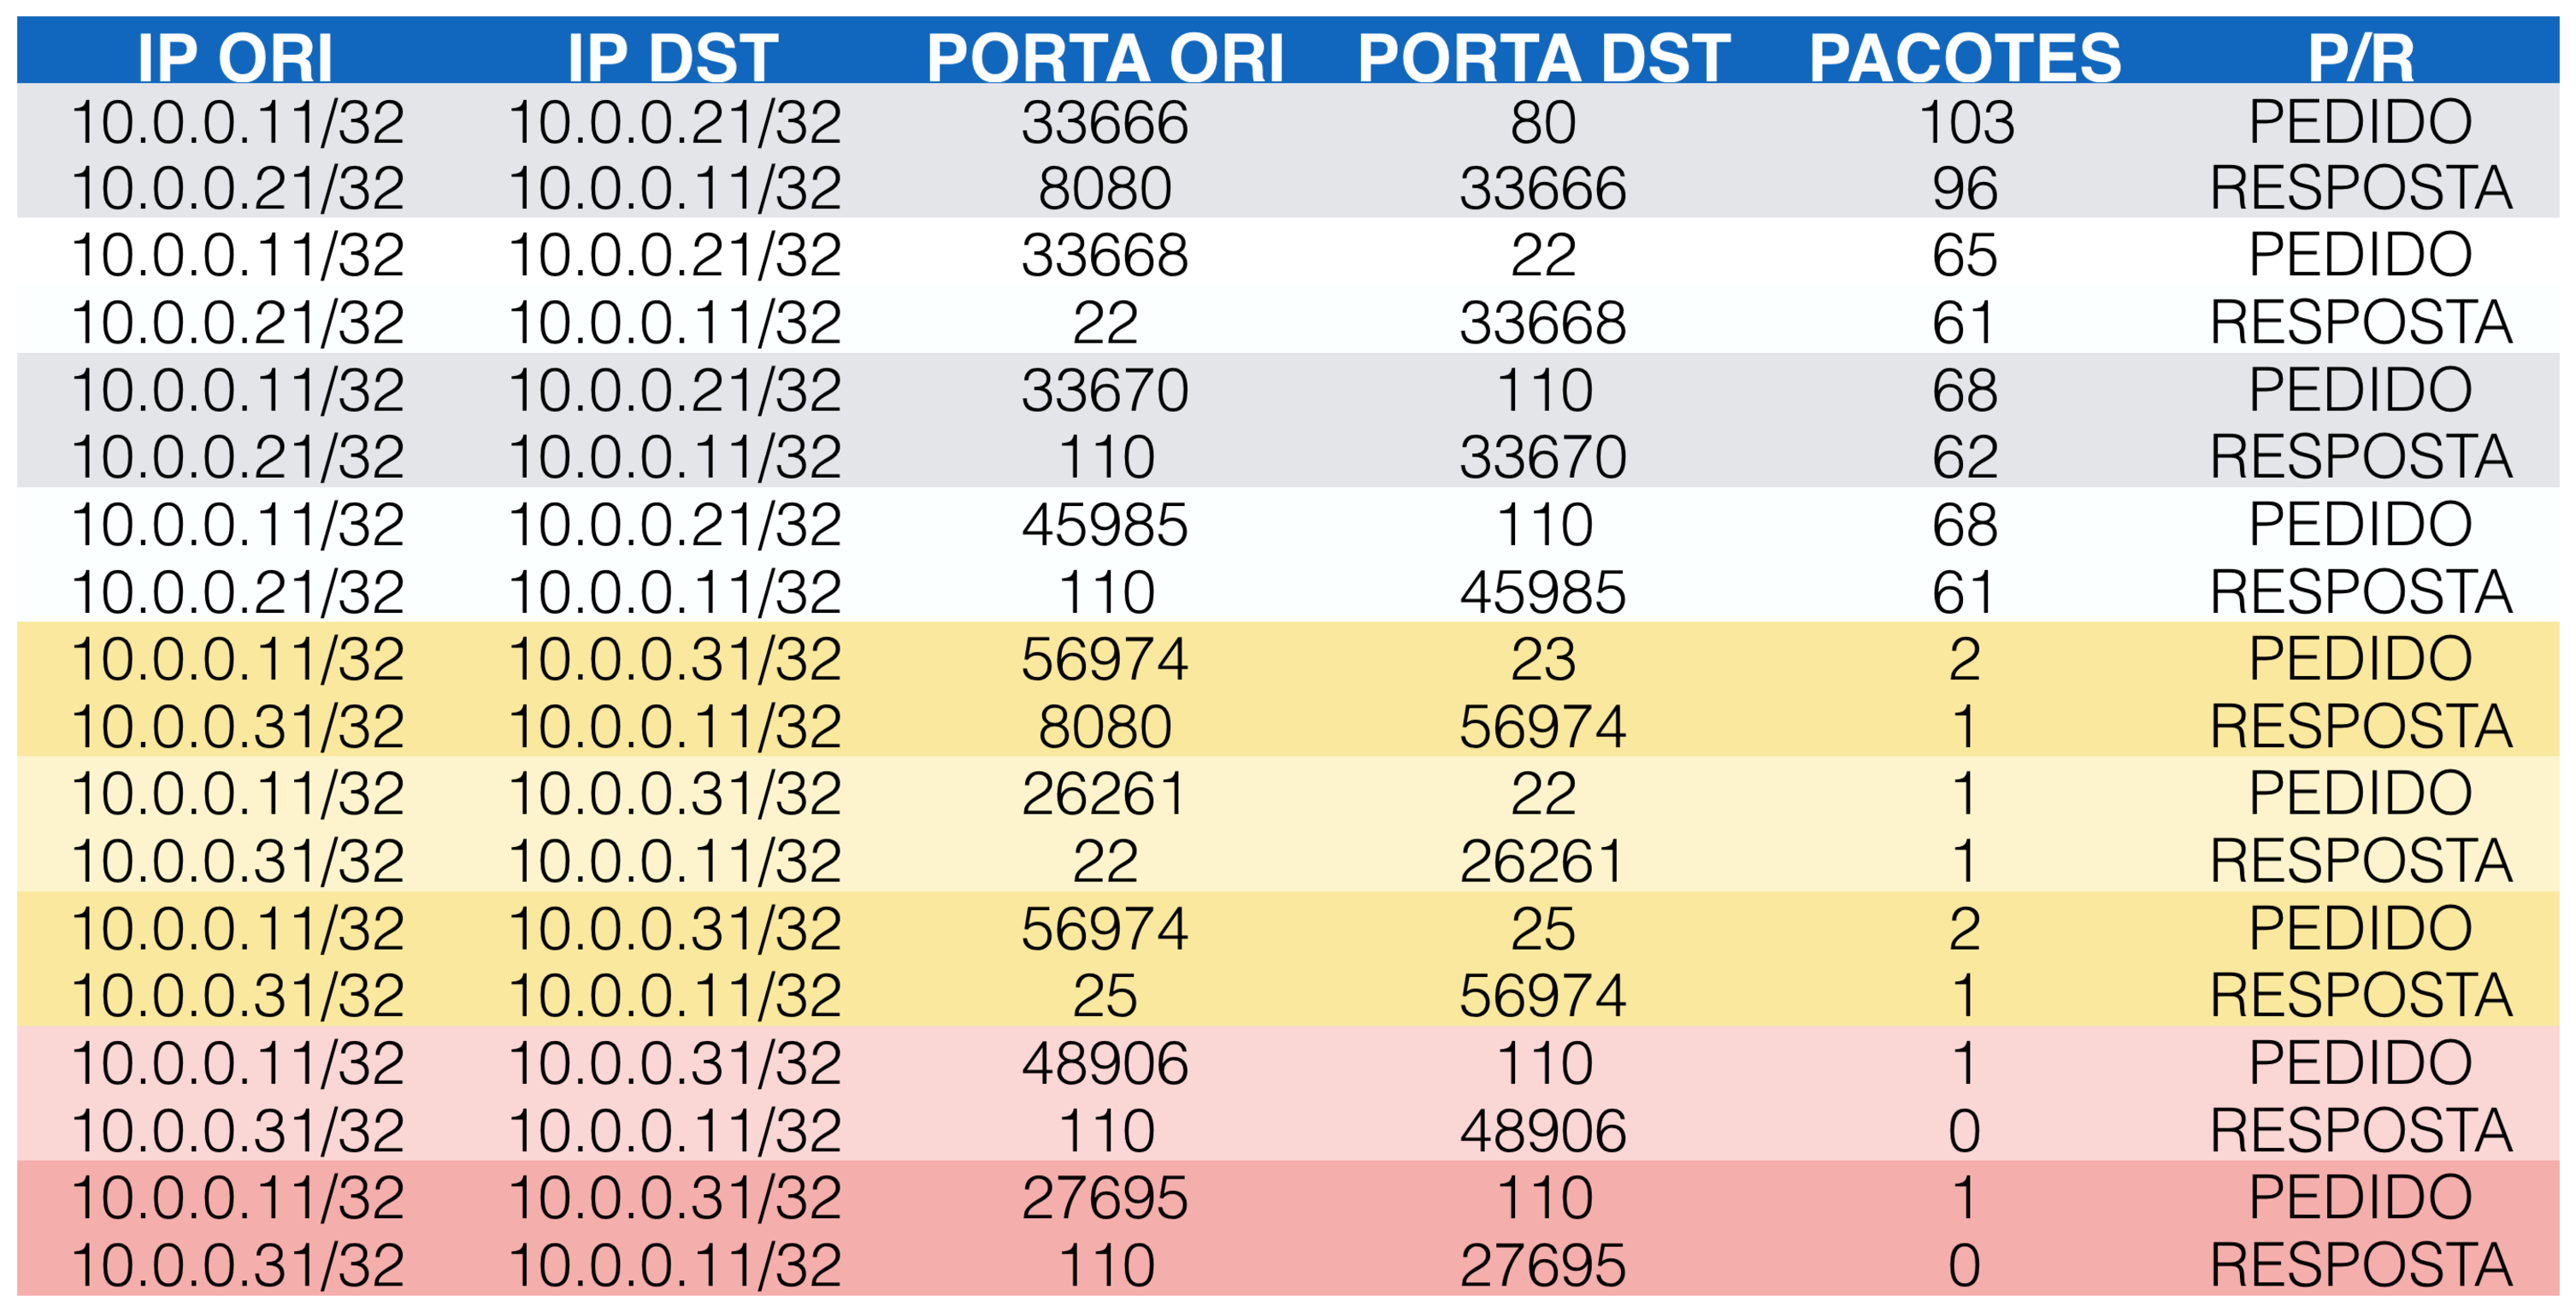
\includegraphics[width=.9\textwidth]{images/base.eps}
  \fonte{Elaborado pelo autor.}
  \label{fig:base}
\end{figure}
\FloatBarrier

O Quadro \ref{fig:e1} apresenta uma análise quantitativa dos fluxos. Em sua segunda coluna são exemplificados os fluxos não maliciosos. Do total de 200.000 fluxos gerados, todos foram encaminhados, não apresentando falsos negativos. A terceira coluna apresenta os resultados da varredura horizontal, onde o comando "nmap -p" foi utilizado com a mesma porta para diferentes \textit{hosts}. Sendo assim, cada um dos quatro computadores tentou varrer os cinco servidores disponíveis o que originou vinte fluxos.

Como a validação é realizada após a varredura de três \textit{hosts} distintos, a quantidade máxima de fluxos maliciosos a ser encaminhado esperada é de 12 fluxos, três por computador (\textit{host} origem). Contudo, a análise resultou em uma quantidade de fluxos igual a 14. Isto ocorreu devido a retransmissão de alguns pacotes, aumentando a quantidade de pacotes por fluxo, e assim, sendo identificados como não maliciosos. Estes fluxos passaram a ser considerados maliciosos apenas no quarto ou no quinto \textit{host} verificado, quando o número de pacotes não passou os cinco estabelecidos. Estes valores podem ser visualizados na terceira coluna do Quadro \ref{fig:e1}.

Na quarta coluna, que representa a execução de varredura vertical, foram gerados mil fluxos maliciosos, essa geração, por ter sido automática, foi consideravelmente mais rápida do que o intervalo de coleta, o que acarretou no encaminhamento de 658 fluxos maliciosos. No momento em que o \textit{software} terminou a análise e os endereços foram adicionados na lista de endereços para descarte, o sistema passou a descartar os 342 pacotes restantes. Além disso, essa varredura também teve alguns pacotes duplicados, fazendo com que doze fluxos que deveriam ser considerados maliciosos, fossem encaminhados como fluxo não malicioso.

Na última coluna são apresentados os números referentes à varredura por exploração FIN. Como citado anteriormente, fluxos não iniciados com pacote SYN são imediatamente descartados, isto pode ser comprovado através dos números apresentados. Todos os mil fluxos originados foram descartados.

\begin{table}[H]
\centering
\caption{Resultados das análises de varreduras.}
\label{fig:e1}
\begin{tabular}{|l|c|c|c|c|}
\hline
\multicolumn{1}{|c|}{} & Não maliciosos & TCP Con. Hor. & TCP Con. Ver. & Expl. FIN \\ \hline
Fluxos Gerados         & 200000          & 20      & 1000     & 1000     \\ \hline
Fluxos Encaminhados    & 200000          & 14      & 658      & 0        \\ \hline
Fluxos Bloqueados      & 0              & 8       & 342      & 1000     \\ \hline
Falsos Positivos       & 0              & 0       & 0        & 0        \\ \hline
Falsos Negativos       & 0              & 2       & 12       & 0        \\ \hline
\end{tabular}
\fonte{Elaborado pelo autor.}
\end{table}

O mesmo procedimento acima realizado foi novamente executado a fim de verificar se de fato todos os fluxos foram adicionados na lista de endereços para descarte. Neste procedimento a lista de endereços para descarte não foi limpa e o resultado encontra-se no Quadro \ref{fig:e2}. Neste pode-se observar que todos os fluxos gerados, inclusive os não maliciosos, foram descartados. Isto é resultado da análise das varreduras anteriores onde todos os \textit{hosts} efetuaram ataques de varredura e foram adicionados na lista para descarte.

\begin{table}[H]
\centering
\caption{Resultados das análises de varreduras após estabelecido o descarte.}
\label{fig:e2}
\begin{tabular}{|l|c|c|c|c|}
\hline
\multicolumn{1}{|c|}{} & Não maliciosos & TCP Con. Hor. & TCP Con. Ver. & Expl. FIN \\ \hline
Fluxos Gerados         & 200000          & 20      & 1000     & 1000     \\ \hline
Fluxos Encaminhados    & 0               & 0      & 0      & 0        \\ \hline
Fluxos Bloqueados      & 200000         & 20       & 1000      & 1000     \\ \hline
Falsos Positivos       & 0              & 0       & 0        & 0        \\ \hline
Falsos Negativos       & 0              & 0       & 0       & 0        \\ \hline
\end{tabular}
\fonte{Elaborado pelo autor.}
\end{table}

Através dos testes realizados foram obtidos os seguintes resultados:
\begin{itemize}
    \item Tempo médio de atraso por fluxo de 4 milissegundos. Decorridos pela necessidade da verificação da lista de endereços para descarte e pela adição de regras no controlador;
    \item Nenhum falso positivo. Se deve principalmente pelo fato de não ter sido realizada nenhuma predição para a detecção e sim a validação de fluxos através da quantidade de pacotes;
    \item 0,034\% de falsos negativos. Decorridos devido a quantidade de pacotes retransmitidos. Sendo assim, o que deveria ser um ataque acabou sendo considerado um fluxo normal;
    \item Grande quantidade de varreduras realizadas até que seu bloqueio fosse efetuado. Apesar do algoritmo de detecção ser assertivo na detecção de varreduras, o intervalo entre uma análise e outra permitiu que o atacante pudesse realizar uma grande quantidade de varreduras.
\end{itemize}

\FloatBarrier

Não foi possível estabelecer um comparativo de desempenho com as soluções apresentadas no Capítulo \ref{cap:trabalhos-relacionados}. Isso decorre em virtude dos projetos não apresentarem resultados de suas análises e/ou suas análises não contemplam ataques de varredura de porta. Cabe salientar que os projetos apresentados que possuem detecção de varredura de porta, não possuem proteção contra os mesmos.